\documentclass[usenames,dvipsnames]{beamer} % beamer is the document class for presentation slides

% languages typesetting rules
\usepackage{polyglossia} % handle multiple languages typesetting rules
\setdefaultlanguage{french} % this presentation is in french
\setotherlanguages{english,greek} % this presentation sometimes uses english and greek texts
\newfontfamily\greekfont[Script=Greek]{Linux Libertine O} % we need a special font for greek text
\newfontfamily\greekfontsf[Script=Greek]{Linux Libertine O} % same, but sans serif

% links configuration
\usepackage{hyperref} % commands such as \href, \url, etc.
\hypersetup{
    colorlinks=true,
    linkcolor=,
    urlcolor=Brown
}

% bibliography configuration
\usepackage[backref=true]{biblatex} % bibliography handling
\newcommand{\titlecite}[1] {
    % Insert the (short) title of the citation, and a reference to it
    \citetitle{#1}\cite{#1}
}

% Configuration to nicely display code examples
\usepackage[skins,minted]{tcolorbox} % fancy colored boxes
\tcbset{ % configure the boxes style
    enhanced, % fancier boxes
    drop shadow,
    overlay={%
        % Add a small darker column to the left of the boxes to receive line numbers
        \begin{tcbclipinterior}
            \fill[gray!25] (frame.south west) rectangle ([xshift=4mm]frame.north west);
        \end{tcbclipinterior}
    }
}
\newmintedfile[texinput]{latex}{ % Shorthand for displaying latex code from file
    linenos, % display line numbers
    numbersep=2mm, % by default line numbers are too far on the left and leave the color box, make them closer
    fontsize=\footnotesize, % make the code smaller
    breaklines=true % break lines if they are too long
}
\newcommand{\texinputbox}[2]{
    % Display latex code through minted inside a color box
    \begin{tcolorbox}[title=#1]
        \selectlanguage{english}
        \texinput{#2}
    \end{tcolorbox}
}
\definecolor{lightlightgray}{gray}{0.93}
\newmintinline[texinline]{latex}{bgcolor=lightlightgray} % Shorthand for \mintinline{latex}{…}
\newmintedfile[shellinput]{shell-session}{ % Shorthand for displaying shell sessions from file
    fontsize=\footnotesize, % make the code smaller
    breaklines=true, % break lines if they are too long
}
\newcommand{\shellinputbox}[2]{
    % Display shell session through minted inside a color box
    \begin{tcolorbox}[title=#1,overlay=]
        \selectlanguage{english}
        \shellinput{#2}
    \end{tcolorbox}
}

\usepackage{csquotes} % biblatex extensions for non-english languages
\usepackage{tipa} % International Phonetic Alphabet symbols and helpers
\usepackage{caption} % more control over captions
\usepackage{ccicons} % icons for Creative-Commons licenses
\usepackage{hologo} % tex and co. logos

% Beamer theme configuration
\usetheme{Warsaw}
\useoutertheme{infolines} % Display the slides number in the footline (and a smaller header)

% Add a tableofcontent slide before each subsection, highlighting the section we're at
\AtBeginSection[]{
    \frame{\tableofcontents[currentsection]}
}

% define the \ipa command that switches to english typography rules before
% calling \textipa (which gets confused by french typography rules)
\newcommand{\ipa}[1] {
    \selectlanguage{english}
    \textipa{#1}
}

% Bibliography configuration
\bibliography{references}

% Meta information about this presentation
\title{Écriture de documents avec \LaTeX{}}
\subtitle{\texorpdfstring{\small{\emph{D'après une conférence de Didier Verna}\cite{latexDV}}}
                         {D'après une conférence de Didier Verna}}
\titlegraphic{\large{\href{https://creativecommons.org/licenses/by-sa/4.0/}{\ccbysa}}}
\institute[]{EPITA Strasbourg}
\author[Paul Hervot]{
    % The authors information appear in the first page of the document but also
    % in the pdf's metadata. A lot of stuff isn't allowed in the metadata
    % (links, line breaks, etc.) so we must define two alternatives, one for the
    % document page and one for the metadata, this is done with the
    % \texordpdfstring command
    \texorpdfstring
    { % Nicely formatted author information
        Paul Hervot\\
        \href{mailto:paul.hervot@epita.fr}{\nolinkurl{paul.hervot@epita.fr}}
    }{ % A simpler version for the pdf's metadata
        Paul Hervot
    }
}
\date{3 septembre 2019}

\begin{document}

\frame{\titlepage{}}

\section{Introduction}
\subsection{\TeX}
\begin{frame}{\TeX}
    \begin{description}
        \item[Nom :] symbolise les lettres \textgreek{τεχ}, abbréviation de \textgreek{τέχνη}
        \item[Objectif :] mise en forme typographique entièrement informatique
        \item[Création :] Donald Knuth, 1977-1989
        \item[Prononciation :] \ipa{[tEx]}
    \end{description}

    \begin{figure}[position]
        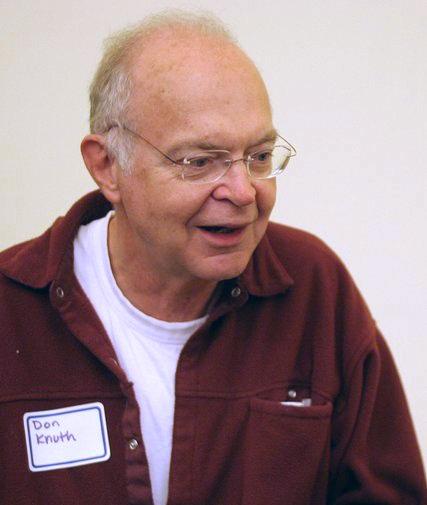
\includegraphics[height=0.5\textheight]{img/knuth}
        \caption*{Donald Knuth, en 2005\cite{knuthpic}}
    \end{figure}
\end{frame}

\subsection{\LaTeX}
\begin{frame}{\LaTeX}
    \begin{description}
        \item[Nom :] abbréviation de Lamport-\TeX
        \item[Objectif :] ensemble de macros (raccourcis) pour \TeX
        \item[Création :] Leslie Lamport, 1983
        \item[Prononciation :] \ipa{["lA:tEx]} ou \ipa{["leI:tEx]}
    \end{description}

    \begin{figure}[position]
        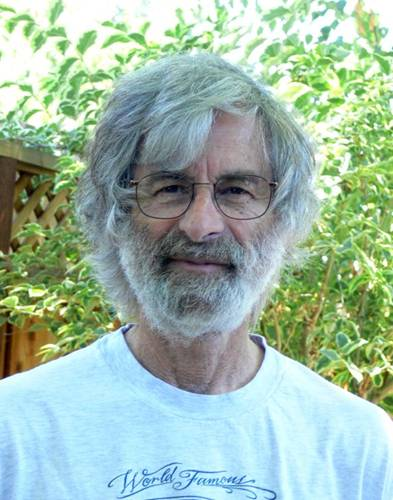
\includegraphics[height=0.5\textheight]{img/lamport}
        \caption*{Leslie Lamport, vers 2014}
    \end{figure}
\end{frame}

\begin{frame}{Intérêts aujourd'hui}
    \begin{itemize}
        \item édition mathématique ;
        \item gestion de bibliographie ;
        \item écriture sous forme de code source distribuable ;
        \item totalement libre, extensible et personnalisable ;
        \item très utilisé dans le milieu de la recherche.
    \end{itemize}
\end{frame}

\begin{frame}{Obtenir \LaTeX}
    \begin{description}
        \item[Multi-plateforme :] \href{http://tug.org/texlive/}{\TeX{}Live}.
            Standard \emph{de facto}, disponible dans toutes les distribution
            Linux.
        \item[Windows :] \href{https://miktex.org/}{\hologo{MiKTeX}}.
        \item[MacOS :] \href{https://www.tug.org/mactex/}{Mac\TeX}, basé sur \TeX{}Live.
        \item[En ligne :] \href{https://www.overleaf.com/}{Overleaf}, payant avec version d'essai.
    \end{description}

    \vspace{1cm}
    Il existe aussi de nombreux IDEs\footnote{Environnement de Développement
    Intégré} comme \href{https://www.xm1math.net/texmaker/}{\TeX{}Maker} et des
    plugins pour éditeurs comme \href{https://github.com/lervag/vimtex}{vimtex}.
    \LaTeX{} étant libre, il existe un très grand nombre d'outils autour.
\end{frame}

\section{Principes fondamentaux}
\subsection{Le langage}
\begin{frame}[fragile]{Organisation de la source d'un document \LaTeX}
    \texinputbox{article.tex}{examples/article-skeleton.tex}

    Anatomie d'une commande : \texinline{\nom[options]{arguments}}
\end{frame}

\begin{frame}[fragile]{Subtilités syntaxiques}
    \begin{itemize}
        \item Plusieurs caractères blancs $\Leftrightarrow$ un seul caractère blanc ;
        \item une ligne blanche $\Rightarrow$ changement de paragraphe ;
        \item caractères spéciaux à "échapper" par un \textbackslash{} :\\
            \texinline{\# \$ \% \^ \& \_ \{ \} \~}
        \item sauf pour \textbackslash{} qui s'écrira
            \texinline{\textbackslash{}} (car \texinline{\\}
            signifie "nouvelle ligne") ;
        \item commentaires : \texinline{%} jusqu'à la fin de la ligne
    \end{itemize}
\end{frame}

\begin{frame}[fragile]{Exemples}
    \begin{columns}
        \begin{column}{0.58\textwidth}
            \texinputbox{exemple.tex}{examples/basics-syntax.tex}
        \end{column}

        \begin{column}{0.43\textwidth}
            \begin{tcolorbox}[title=exemple.pdf, overlay=]
                Le nombre d'espaces     ne  compte
    pas
    dans le
	fichier source.

Les commentaires % sont totalement
% ignorés par le compilateur
Les utili% ils annulent des espaces
   sateurs de \TeX{} aiment faire
des jeux de mots, ils s'appellent
parfois:\\ les \TeX{}niciens, les
\TeX perts, etc\ldots

            \end{tcolorbox}
        \end{column}
    \end{columns}

    \begin{columns}
        \begin{column}{0.58\textwidth}
            \begin{tcolorbox}[overlay=]
                \footnotesize
                \texinline[bgcolor=]{\^o, \c c, \c C, \oe, \` A, \" i}
            \end{tcolorbox}
        \end{column}

        \begin{column}{0.43\textwidth}
            \begin{tcolorbox}[overlay=]
                \^o, \c c, \c C, \oe, \` A, \" i
            \end{tcolorbox}
        \end{column}
    \end{columns}
\end{frame}

\subsection{Compilation}
\begin{frame}[fragile]{\hologo{pdfTeX}}
    \shellinputbox{Avec l'outil \hologo{pdfLaTeX}}{examples/session-pdflatex.session}

    Peut être l'outil le plus connu.
\end{frame}

\begin{frame}[fragile]{\hologo{XeTeX}}
    \shellinputbox{Avec l'outil \hologo{XeLaTeX}}{examples/session-xelatex.session}

    Une meilleur gestion de l'unicode et des polices modernes.
\end{frame}

\section{Fonctionnalités du langage}
\subsection{Configuration globale du document}
\begin{frame}[fragile]{Les classes de document}
    La classe d'un document est définiée par la commande:

    \texinputbox{}{examples/documentclass-struct.tex}

    \begin{description}
        \item[Lettre :] \texinline{\documentclass[a4paper]{letter}}\\
            \textrightarrow{} \texinline{\signature{…}}, \texinline{\address{…}},
            etc…
        \item[Article :] \texinline{\documentclass{article}} \vspace{-5pt}
        \item[Rapport :] \texinline{\documentclass{report}} \vspace{-5pt}
        \item[Livres :] \texinline{\documentclass{book}}\\
            \textrightarrow{} \texinline{\title{…}}, \texinline{\author{…}}, etc…
        \item[Présentations :] \texinline{\documentclass{beamer}}\\
            \textrightarrow{} \texinline{\begin{frame}},
                \texinline{\usetheme{…}}, etc…
    \end{description}
\end{frame}

\begin{frame}[fragile]{Les paquets}
    Ajoutent des fonctionnalités (surtout des commandes) disponibles. Ils sont
    inclus avec:

    \texinputbox{}{examples/usepackage-struct.tex}

    \begin{description}
        \item[Liens cliquables:]
            \texinline{\usepackage[colorlinks=true]{hyperref}}\\
            \textrightarrow{} \texinline{\href{…}{…}}, \texinline{\url{…}}, etc…
        \item[Cadres colorés:] \texinline{\usepackage{tcolorbox}}\\
            \textrightarrow{} \texinline{\begin{tcolorbox}},
                \texinline{\tcbset{…}}, etc…
        \item[Coloration syntaxique:] \texinline{\usepackage{minted}}\\
            \textrightarrow{} \texinline{\begin{minted}{python}},
            \texinline{\mintinline{ocaml}{…}}, etc…
    \end{description}

    Et \emph{beaucoup} d'autres.
\end{frame}

\begin{frame}[fragile]{Internationalisation (i18n)}
    Avec le paquet Babel:
    \texinputbox{}{examples/babel-fr.tex}

    Enjeux:
    \begin{itemize}
        \item respect automatique des règles de typographie (espaces devant les
        signes de ponctuation, césures, …);
        \item localisation des textes automatiques ("Table des matières",
        "Bibliographie", …);
        \item encodage et jeu de caractères du fichier source (voir aussi
        \texinline{\usepackage[utf8]{inputenc}}).
    \end{itemize}

    Il est aussi possible de gérer plusieurs langages dans un même document et
    de passer de l'un à l'autre avec des commandes (voir aussi
    \texinline{\usepackage{polyglossia}}).
\end{frame}

\begin{frame}[fragile]{Quelques éléments typographiques}
    \begin{columns}
        \begin{column}{0.50\textwidth}
            \texinputbox{exemple.tex}{examples/typo-examples.tex}
        \end{column}

        \begin{column}{0.50\textwidth}
            \begin{tcolorbox}[title=exemple.pdf, overlay=]
                Points de suspension: ..., …
ou \ldots\\

Faire ressortir quelque chose
d'\emph{important}.\\

Plusieurs types de tirets:\\
porte-manteau\\
pages 13--27\\
--- Je suis Paul\\
--- Et moi Antoine!

            \end{tcolorbox}
        \end{column}
    \end{columns}
\end{frame}
\section{Conclusion}
\subsection{Autres ressources et références}
\begin{frame}{Autre documentation}
    \begin{description}
        \item[Livres]{
            \begin{itemize}
                \item \titlecite{lamport1994latex}
                \item \titlecite{goossens1997latex}
                \item \titlecite{rolland1999latex}
            \end{itemize}
        }
        \item[En ligne]{
            \begin{itemize}
                \item \titlecite{oetiker2011not}
                \item \url{http://www.latex-project.org}
                \item \url{http://www.ctan.org} (le "\textenglish{Comprehensive
                    \TeX{} Archive Network}", documentation complète de toutes
                    les extensions)
                \item \url{https://tex.stackexchange.com} (forum de
                    question/réponses)
                \item \url{https://en.wikibooks.org/wiki/LaTeX}
            \end{itemize}
        }
    \end{description}
\end{frame}
\begin{frame}[allowframebreaks]{Bibliographie}
    \printbibliography{}
\end{frame}
\end{document}
